\documentclass{article}
\usepackage{dirtytalk}
\usepackage[utf8]{inputenc}
\usepackage[acronym]{glossaries}
\usepackage{pgfgantt}
\usepackage{hyperref}
\usetikzlibrary{arrows.meta,
                chains,
                positioning}
\hypersetup{
    colorlinks=true,
    linkcolor=black,
    filecolor=black,      
    urlcolor=black,
    citecolor=black,
    pdftitle={Thesis Proposal},
    pdfpagemode=FullScreen,
}
\makeglossaries

\newacronym{hei}{CHEI}{Colorado Higher Education Institution}
\newacronym{heis}{CHEIs}{Colorado Higher Education Institutions}
\newacronym{wcag}{WCAG}{Web Content Accessibility Guidelines}
\newacronym{w3c}{W3C}{World Wide Web Consortium}
\newacronym{wai}{WAI}{Web Accessibility Initiative}
\newacronym{ada}{ADA}{Americans with Disabilities Act}

\title{Thesis Proposal: Digital Accessibility in Colorado Higher Education Institutions}
\author{Eryn Kelsey-Adkins\\Computer Science Department\\Colorado School of Mines}
\date{January 2022}

\begin{document}

\maketitle

\tableofcontents

\section{Overview}

Digital accessibility is an important part of increasing diversity and inclusion in higher education; however there has been no comprehensive review of digital accessibility in \acrfull{heis}. In order to properly identify areas of improvement, a baseline of current digital accessibility must be evaluated. 

This research proposal suggests an approach to create this baseline in digital accessibility by evaluating \acrshort{hei} web content according to \acrfull{wcag} through both automated and manual testing, and interviewing instructional accessibility experts and students who are affected by a lack of digital accessibility.

As today's computer science students are tomorrow's digital accessibility experts, it is important to understand when and where accessibility is taught in the classroom. Therefore a series of surveys of current computer science students and instructors is further proposed.

\section{Background}

Digital accessibility, or web content accessibility, commonly refers to removing and/or preventing barriers to interactions with, or access to, websites and digital tools by people with disabilities \cite{george}. According to the CDC, 26\% of American adults have some sort of disability. Of those, 13.7\% have mobility issues, 10.8\% have difficulty concentrating, remembering, or making decisions, 5.9\% have hearing loss, and 4.6\% have low or no vision \cite{cdc_disability_2019}. All of these disabilities can affect accessing or interacting with digital content. Prioritizing digital accessibility prioritizes inclusion and diversity.

\acrlong{wcag} have been developed under the \acrfull{w3c} \acrfull{wai}, with a goal of \say{providing a single shared standard for web content accessibility that meets the needs of individuals, organizations, and governments internationally.} \cite{wcag_intro}

\acrshort{wcag} are developed collaboratively with an active community of developers, accessibility experts, and advocates. The current success criteria are \acrshort{wcag} 2.1, although \acrshort{wcag} 2.2 criteria are scheduled to be published in June of this year \cite{wai_develop}.
\vspace{2em}

    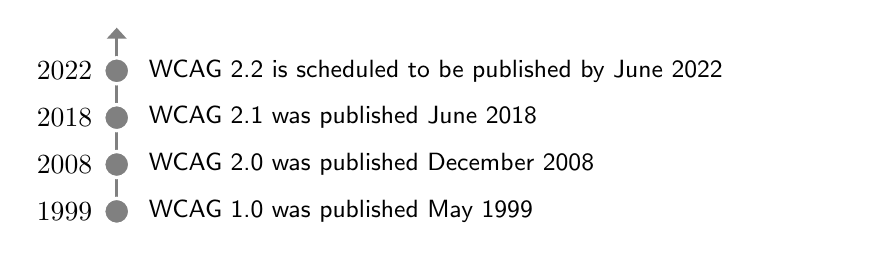
\begin{tikzpicture}[
node distance = 1mm and 3mm,
  start chain = A going below,
   dot/.style = {circle, draw=white, very thick, fill=gray,
                 minimum size=3mm},
   box/.style = {rectangle, text width=85mm,
                 inner xsep=4mm, inner ysep=1mm,
                 font=\sffamily\small\linespread{0.84}\selectfont,
                 on chain},
                        ]
    \begin{scope}[every node/.append style={box}]
\node { WCAG 2.2 is scheduled to be published by June 2022} ;
\node { WCAG 2.1 was published June 2018} ;
\node { WCAG 2.0 was published  December 2008} ;
\node { WCAG 1.0 was published May 1999} ;

    \end{scope}
\draw[very thick, gray, {Triangle[length=4pt)]}-{Circle[length=3pt]},
      shorten <=-3mm, shorten >=-3mm]           % <--- here is adjusted additional arrow's 
    (A-1.north west) -- (A-3.south west);
\foreach \i [ count=\j] in {2022,2018,2008,1999}
    \node[dot,label=left:\i] at (A-\j.west) {};
    \end{tikzpicture}
\vspace{2em}

\acrshort{wcag} success criteria are based on the four principles of accessibility: content must be Perceivable, Operable, Understandable, and Robust (POUR). According to \acrshort{w3c}, these principles are defined as: 

\begin{enumerate}
    \item Perceivable: information must be presented to users in ways they can perceive, regardless of disability.
    \item Operable: the interface and navigation must be operable by all.
    \item Understandable: both content and interface components must be understandable.
    \item Robust: a wide variety of of both user agents and assistive technologies must be able to interpret the content. \cite{wcag}
\end{enumerate}


Higher Education Institutions should be bastions of digital accessibility. However, very few university and college websites meet the \acrshort{wcag} 2.1 criteria \cite{empirical}. Not only does this have ethical implications, it may run afoul of the law. Section 508 and the \acrfull{ada} applies to public colleges and universities under Title II, and to private colleges and universities under Title III, if they receive any federal funds. Section 508 mandates that all electronic communication must be accessible to persons with disabilities \cite{508}. Note that accessibility is different than accommodation. Accommodations are specific to a student and their disability. Accessibility is general and should be proactive.

Identifying and highlighting areas in public facing websites that do not meet current \acrshort{wcag} 2.1 criteria is the first step to ensuring accessibility of digital content in \acrshort{heis}. Most, if not all, institutions have instructional accessibility experts that assist in creating accessible instructional content. Interviews with these experts and with students with disabilities will identify pain points in instructional accessibility. Finally, just as accessibility should be proactive, Computer Science Departments must also be proactive in teaching students accessibility concepts. In informal discussions with computer science students in \acrshort{heis} across the state, very few were aware of digital accessibility and how their future work can affect it. Further research will show how and when accessibility is taught in \acrshort{heis} and may reveal areas for improvement in Computer Science education. 

\section{Proposed Methodology}

This project aims to evaluate digital accessibility in \acrlong{heis} three ways:

\begin{enumerate}
    \item Testing public facing websites according to \acrshort{wcag} 2.1 AA criteria.
    \item Interviewing subject matter experts in instructional accessibility.
    \item Surveying current Computer Science students and instructors on when and where accessibility is taught in the curriculum.
\end{enumerate}

\subsection{Identifying \acrlong{heis}}

The Colorado Department of Higher Education maintains a list of Colorado Colleges and Universities available on their website \cite{cdhe}. For the purposes of this research, \acrlong{heis} will be defined as these institutions.

\subsection{\acrlong{wcag}}

\acrshort{heis} will be tested according to \acrshort{wcag} 2.1 AA success criteria, which is Section 508 compliant \cite{wcag}. Evaluation will be completed through a mix of automated, semi-automated, and manual testing.

\subsubsection{Automated Testing}

A number of automated testing tools are available; \acrshort{w3c} maintains a list of both automated and semi-automated tools on their website \cite{tools}. Acosta-Vargas et al. evaluated AccessMonitor, AChecker, eXaminator, TAW, Tenon, WAVE and Web Accessibility Checker \cite{acosta}. Abascal et al. evaluated AChecker, Mauve, WAVE, TAW, Tenon, aDesigner, Continuous Accessibility Testing for Eclipse, and Accessibility checker for CKEditor 4 \cite{abascal}. Deque has published the axe API which can be used to create automated testing with languages such as Python (Selenium, Beautiful Soup), or JavaScript (Node.js) \cite{axe}.

A selection of automated and semi-automated testing will be evaluated for accuracy, ease of use, and applicability to the project. Once identified, the best tool or tools will be used to gather quantitative data on accessibility errors.

\subsubsection{Manual Testing}

Automated and semi-automated testing makes accessibility evaluation faster and easier, but it cannot replace the human element. An automated tool cannot evaluate alternative text for appropriateness or if media query resizing affects readability. See Figure \ref{fig:csm} for an example from mines.edu.

\begin{figure}[h]
    \centering
    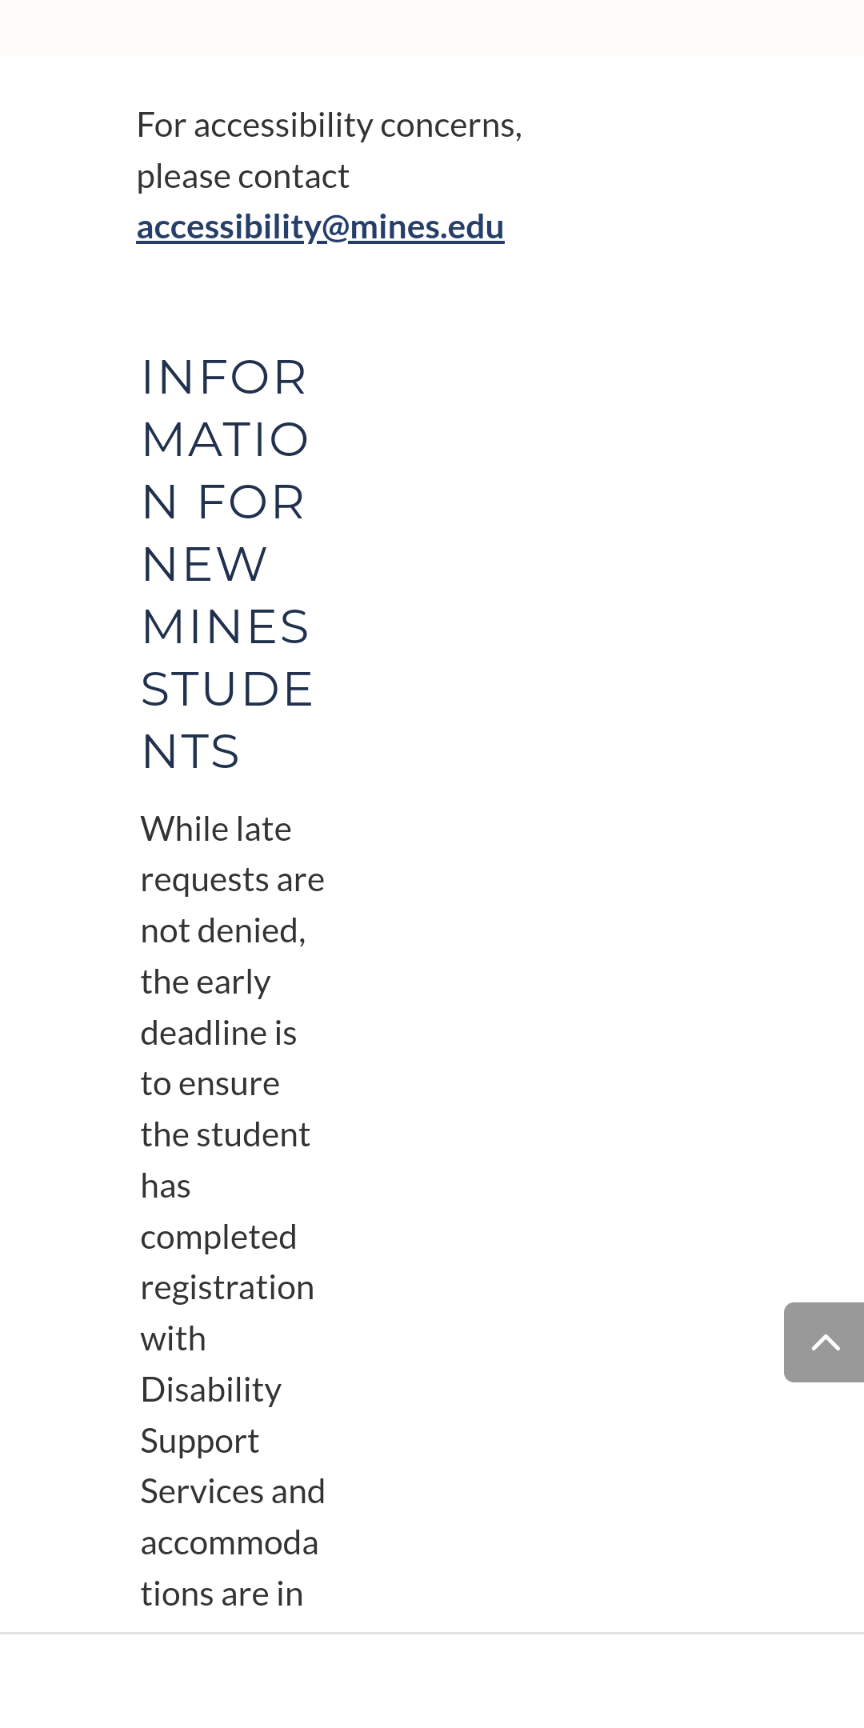
\includegraphics[width=0.3\textwidth]{Screenshot_20220111-161636.png}
    \caption{A screenshot from the Colorado School of Mines website showing how media query resizing affects readability}
    \label{fig:csm}
\end{figure}

A sample size of web pages will be determined for manual testing, and common tasks, such as finding the semester start date, lists of clubs and activities, or admissions requirements, will be identified for user testing by persons with disabilities.

\subsection{Interviews with Subject Matter Experts}

Interviews with \acrshort{hei} website developers, instructional accessibility experts, disability services, and students with disabilities will be conducted and evaluated with grounded theory. 

\subsection{Surveys}

Current Computer Science students and instructors at \acrshort{heis} will be surveyed to discover when and how accessibility in web content and graphical user interfaces is taught. 

\section{Research Plan}

A tentative timeline of the research plan is below. See Figure \ref{fig:gantt1} for a visualization of this timeline.

\begin{enumerate}
    \item Literature review
    \begin{itemize}
        \item Approximately 2 months
        \item January - February 2022
    \end{itemize}
    \item Database Design
    \begin{itemize}
        \item Approximately 2 weeks
        \item Will overlap with other tasks
        \item January 2022
    \end{itemize}
        \item Generating list of web addresses for testing
    \begin{itemize}
        \item Approximately 2 weeks
        \item Will be automated
        \item January 2022
    \end{itemize}
    \item Automated tool review
    \begin{itemize}
        \item Approximately 1 month
        \item Will overlap with literature review
        \item February 2022
    \end{itemize}
    \item Needfinding interviews
    \begin{itemize}
        \item Approximately 2 months
        \item April - May 2022
    \end{itemize}
    \item Grounded theory analysis
    \begin{itemize}
        \item Approximately 2 months
        \item May - June 2022
    \end{itemize}
    \item Automated testing
    \begin{itemize}
        \item Approximately 3 months
        \item April - June 2022
    \end{itemize}
    \item Manual testing
    \begin{itemize}
        \item Approximately 6 weeks
        \item July - August 2022
    \end{itemize}
    \item Surveys
    \begin{itemize}
        \item Approximately 2 months
        \item August - September 2022
    \end{itemize}
    \item Data Analysis
    \begin{itemize}
        \item Approximately 2 months
        \item September - October 2022
    \end{itemize}
    \item Writing
    \begin{itemize}
        \item Approximately 4 months
        \item November 2022 - February 2023
    \end{itemize}
    \item Review and Revisions
    \begin{itemize}
        \item Approximately 2 months
        \item April - May 2023
    \end{itemize}
\end{enumerate}

\begin{figure}[h]
    \centering
    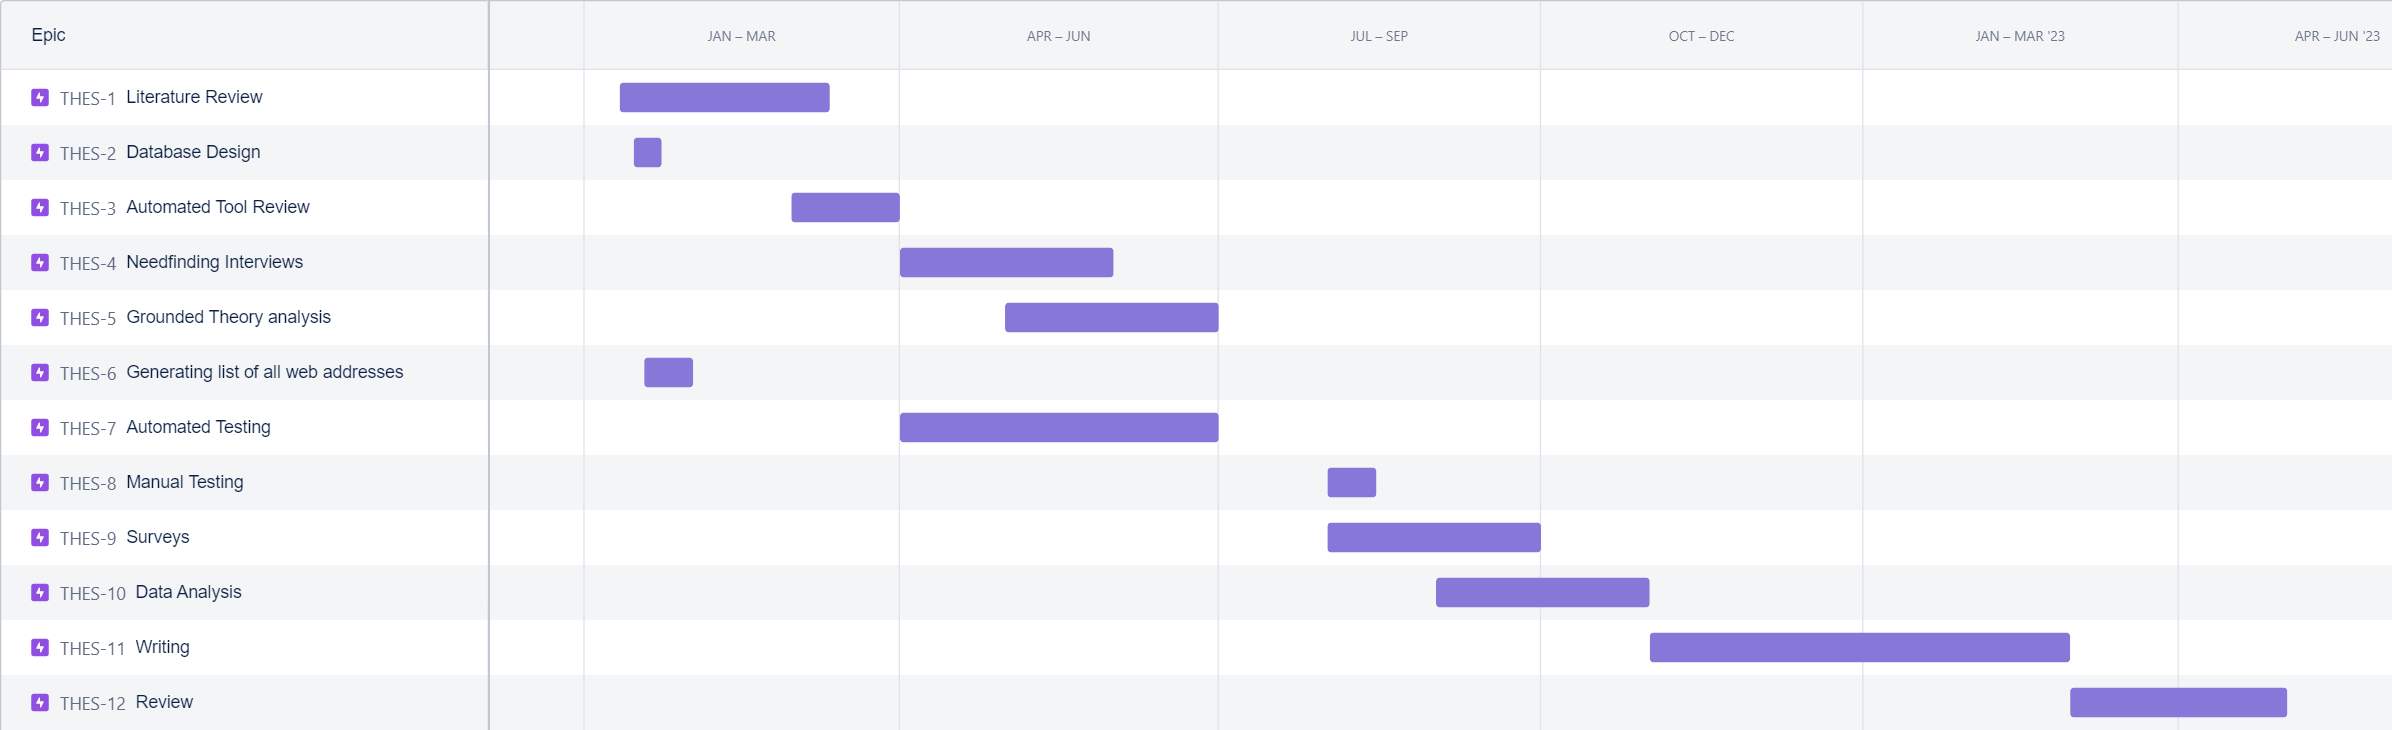
\includegraphics[width=\textwidth]{thesis_2022-01-11_05.54pm.png}
    \caption{A Gantt chart visualizing the research plan timeline}
    \label{fig:gantt1}
\end{figure}

Note that this timeline is tentative and may be adjusted. The project milestones will be tracked through Jira. 

\printglossary

\bibliographystyle{IEEEtran}
% argument is your BibTeX string definitions and bibliography database(s)
\bibliography{refs}
\end{document}
